\chapter{Perhitungan Aljabar dan Persamaan}\label{ch:g8:equations}

Kelas 7 memperkenalkan huruf lalu menyederhanakan bentuk yang
sederhana (\cref{ch:g7:literal}). Bab ini menambahkan dua keterampilan
yang membuat aljabar menjadi kuat: \emph{menjabarkan} \omterm{def:g2:mult:def}{hasil kali} tanda
kurung, dan \emph{menyelesaikan \omterm{def:g8:equations:def}{persamaan}} --- mencari bilangan yang
bersembunyi di balik hurufnya.

\section{Menjabarkan}

\begin{theorem}[Sifat distributif tunggal dan ganda]\label{thm:g8:equations:expand}
Untuk semua bilangan:
\[
k(a + b) = ka + kb,
\qquad
(a + b)(c + d) = ac + ad + bc + bd .
\]
\end{theorem}

\begin{proof}
Aturan yang pertama adalah \cref{thm:g7:priorities:distributivity}
(termasuk tandanya: $k$ dan sukunya boleh negatif,
\cref{ch:g8:negprod}). Untuk yang kedua, terapkan aturan pertamanya
dua kali, dengan memperlakukan $(c + d)$ sebagai satu bilangan:
\[
(a + b)(c + d) = a(c + d) + b(c + d) = ac + ad + bc + bd .
\qedhere
\]
\end{proof}

\begin{example}\label{ex:g8:equations:expand}
Perhatikan tandanya pada tiap sukunya:
\begin{align*}
3(2x - 5) &= 6x - 15, \\
-2(4x - 7) &= -8x + 14
&& \text{(minus membalik kedua tandanya)}, \\
(x + 3)(x + 5) &= x^2 + 5x + 3x + 15 = x^2 + 8x + 15, \\
(2x - 1)(x - 4) &= 2x^2 - 8x - x + 4 = 2x^2 - 9x + 4 .
\end{align*}
\end{example}

\begin{omfigure}
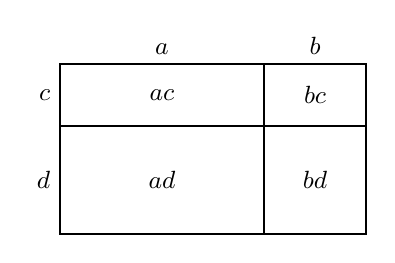
\begin{tikzpicture}[scale=0.72]
  \draw[thick] (0,0) rectangle (5.4,3.0);
  \draw[thick] (3.6,0) -- (3.6,3.0);
  \draw[thick] (0,1.9) -- (5.4,1.9);
  \node[font=\small] at (1.8,2.45) {$ac$};
  \node[font=\small] at (4.5,2.45) {$bc$};
  \node[font=\small] at (1.8,0.95) {$ad$};
  \node[font=\small] at (4.5,0.95) {$bd$};
  \node[above, font=\small] at (1.8,3.0) {$a$};
  \node[above, font=\small] at (4.5,3.0) {$b$};
  \node[left, font=\small] at (0,2.45) {$c$};
  \node[left, font=\small] at (0,0.95) {$d$};
\end{tikzpicture}

{\small Sifat distributif ganda sebagai luas: persegi panjang
$(a+b) \times (c+d)$ terbelah menjadi empat persegi panjang yang lebih
kecil --- satu untuk tiap suku penjabarannya.}
\end{omfigure}

\begin{method}[Menjabarkan dan menyederhanakan]\label{met:g8:equations:reduce}
\begin{enumerate}
  \item Jabarkan setiap \omterm{def:g2:mult:def}{hasil kalinya}, dengan menulis tiap suku
        beserta tandanya;
  \item kumpulkan suku sejenisnya ($x^2$ dengan $x^2$, $x$ dengan
        $x$, bilangan dengan bilangan);
  \item periksalah dengan sebuah nilai: sulihkan misalnya $x = 2$
        pada bentuk aslinya dan pada hasilnya --- hasil yang sama
        menangkap sebagian besar kekeliruan.
\end{enumerate}
\end{method}

\section{Menyelesaikan persamaan}

\begin{definition}[Persamaan]\label{def:g8:equations:def}
\emph{Persamaan}\index{persamaan} adalah kesamaan yang memuat sebuah
bilangan yang belum diketahui, yang ditulis $x$ (atau huruf apa pun).
\emph{Menyelesaikannya} berarti mencari semua nilai $x$ yang membuat
kesamaannya benar --- yaitu \emph{penyelesaiannya}.
\end{definition}

\begin{theorem}[Aturan keseimbangan]\label{thm:g8:equations:balance}
Sebuah \omterm{def:g8:equations:def}{persamaan} tetap punya penyelesaian yang persis sama ketika:
\begin{enumerate}
  \item bilangan yang sama ditambahkan pada (atau dikurangkan dari)
        kedua ruasnya;
  \item kedua ruasnya dikalikan (atau dibagi) dengan bilangan yang
        sama dan \emph{bukan \omterm{def:g1:counting:zero}{nol}}.
\end{enumerate}
\end{theorem}
\admitted

\begin{omfigure}
\begin{tikzpicture}[scale=0.9]
  \draw[thick] (0,0) -- (0,0.5);
  \draw[thick] (-2.6,0.5) -- (2.6,0.5);
  \draw[thick] (-0.5,0) -- (0.5,0);
  \draw[thick] (-2.2,0.5) -- (-2.2,0.75);
  \draw[thick] (2.2,0.5) -- (2.2,0.75);
  \draw[omDef, fill=omDef!15] (-2.8,0.75) rectangle (-1.6,1.45);
  \node[font=\small] at (-2.2,1.1) {$x{+}3$};
  \draw[omThm, fill=omThm!15] (1.75,0.75) rectangle (2.65,1.45);
  \node[font=\small] at (2.2,1.1) {$8$};
  \node[below, font=\small] at (0,-0.25)
    {ambil $3$ dari kedua piringnya: $x = 5$};
\end{tikzpicture}

{\small \omterm{def:g8:equations:def}{Persamaan} adalah neraca yang seimbang: apa pun yang dilakukan
pada satu piringnya harus dilakukan pada piring yang lain, dan
keseimbangannya --- yaitu kesamaannya --- tetap bertahan.}
\end{omfigure}

\begin{method}[Menyelesaikan persamaan berderajat satu]\label{met:g8:equations:solve}
\begin{enumerate}
  \item Jabarkan lalu sederhanakan tiap ruasnya kalau perlu;
  \item tambahkan atau kurangkan pada kedua ruasnya untuk
        mengumpulkan suku $x$ pada satu ruas dan bilangan biasanya
        pada ruas yang lain;
  \item sederhanakan, lalu bagilah kedua ruasnya dengan koefisien
        $x$;
  \item \emph{periksalah} dengan menyulihkan nilai yang ditemukan ke
        dalam \omterm{def:g8:equations:def}{persamaan} aslinya.
\end{enumerate}
\end{method}

\begin{example}\label{ex:g8:equations:solve}
Selesaikan $7x - 5 = 4x + 16$:
\begin{align*}
7x - 5 &= 4x + 16 \\
7x - 4x &= 16 + 5
&& \text{(tambahkan $5$, kurangkan $4x$, pada kedua ruasnya)} \\
3x &= 21 \\
x &= 7 && \text{(bagilah kedua ruasnya dengan 3).}
\end{align*}
Periksa: ruas kirinya $7 \times 7 - 5 = 44$; ruas kanannya
$4 \times 7 + 16 = 44$. Penyelesaiannya adalah $7$.
\end{example}

\begin{example}[Dengan tanda kurung dan bilangan negatif]\label{ex:g8:equations:brackets}
Selesaikan $3(x - 4) = 5 - 2(x + 1)$:
\begin{align*}
3x - 12 &= 5 - 2x - 2 && \text{(jabarkan kedua ruasnya)} \\
3x - 12 &= 3 - 2x && \text{(sederhanakan)} \\
5x &= 15 && \text{(tambahkan $2x + 12$ pada kedua ruasnya)} \\
x &= 3 .
\end{align*}
Periksa: $3(3 - 4) = -3$ dan $5 - 2(3+1) = 5 - 8 = -3$. \quad
Penyelesaiannya: $3$.
\end{example}

\begin{method}[Menyelesaikan soal dengan persamaan]\label{met:g8:equations:problem}
\begin{enumerate}
  \item Pilihlah bilangan yang belum diketahuinya: ``misalkan $x$
        adalah \dots'' (besaran yang ditanyakan, atau besaran lain
        yang lebih sederhana yang berkaitan dengannya);
  \item terjemahkan ceritanya menjadi sebuah \omterm{def:g8:equations:def}{persamaan};
  \item selesaikan \omterm{def:g8:equations:def}{persamaannya};
  \item tafsirkan: jawablah pertanyaan aslinya dalam satu kalimat,
        beserta satuannya, lalu periksalah jawabannya terhadap
        ceritanya.
\end{enumerate}
\end{method}

\begin{example}\label{ex:g8:equations:problem}
Lukas $4$ tahun lebih tua daripada adik perempuannya; bersama-sama
umur mereka berjumlah $26$. Misalkan $x$ umur adiknya; maka umur Lukas
adalah $x + 4$, dan
\[
x + (x + 4) = 26
\ \Longrightarrow\
2x + 4 = 26
\ \Longrightarrow\
2x = 22
\ \Longrightarrow\
x = 11 .
\]
Adiknya berumur $11$, Lukas berumur $15$. Periksa: $11 + 15 = 26$ dan
$15 - 11 = 4$.
\end{example}

\section{Urutan dan pertidaksamaan}

\begin{proposition}[Operasi dan urutan]\label{prop:g8:equations:order}
Menambahkan bilangan yang sama pada kedua ruas sebuah pertidaksamaan
mempertahankannya; mengalikan kedua ruasnya dengan bilangan
\emph{positif} mempertahankannya; mengalikan dengan bilangan
\emph{negatif} \emph{membalikkannya}:
\[
2 < 5 \ \text{ tetapi }\ (-1) \times 2 > (-1) \times 5 .
\]
\end{proposition}
\admitted

\begin{example}\label{ex:g8:equations:inequality}
Selesaikan $5 - 2x \leq 11$: kurangkan $5$ pada kedua ruasnya,
$-2x \leq 6$; bagilah dengan $-2$ \emph{lalu balikkan}: $x \geq -3$.
Semua bilangan yang lebih besar daripada atau sama dengan $-3$ adalah
penyelesaiannya --- \omterm{def:g8:equations:def}{persamaan} biasanya punya satu penyelesaian,
sedangkan pertidaksamaan punya setengah garis penuh penyelesaian.
\end{example}

\section{Latihan}

\begin{exercise}[$\star$]\label{exo:g8:equations:1}
Jabarkan lalu sederhanakan:
\[
5(2x + 3), \qquad
-3(4x - 1), \qquad
2(3x - 2) + 4(x + 5).
\]
\end{exercise}

\begin{exercise}[$\star$]\label{exo:g8:equations:2}
Jabarkan lalu sederhanakan:
\[
(x + 2)(x + 7), \qquad
(3x + 1)(2x - 5), \qquad
(x - 4)(x - 6).
\]
\end{exercise}

\begin{exercise}[$\star$]\label{exo:g8:equations:3}
Apakah $x = 3$ penyelesaian $4x - 5 = 7$? Penyelesaian
$2x + 1 = x + 4$? Penyelesaian $x^2 = 6x - 9$? (Sulihkan lalu
bandingkan kedua ruasnya.)
\end{exercise}

\begin{exercise}[$\star$]\label{exo:g8:equations:4}
Selesaikan, disertai pemeriksaan:
\[
x + 9 = 4, \qquad
5x = -35, \qquad
\frac{x}{3} = 8, \qquad
2x - 7 = 13 .
\]
\end{exercise}

\begin{exercise}[$\star$]\label{exo:g8:equations:5}
Selesaikan:
\[
6x + 5 = 2x + 25, \qquad
9 - 4x = x - 11, \qquad
3(x + 2) = 2x + 11 .
\]
\end{exercise}

\begin{exercise}[$\star$]\label{exo:g8:equations:6}
Selesaikan $4(2x - 3) = 5(x + 6)$, dengan menjabarkannya lebih
dahulu, lalu periksalah penyelesaianmu.
\end{exercise}

\begin{exercise}[$\star$]\label{exo:g8:equations:7}
Terjemahkan lalu selesaikan: ``tiga kali sebuah bilangan, dikurangi
$8$, sama dengan $19$''; ``dua kali sebuah bilangan yang ditambah $5$
sama dengan bilangan itu yang ditambah $12$''.
\end{exercise}

\begin{exercise}[$\star\star$]\label{exo:g8:equations:8}
Panjang sebuah persegi panjang $5$ cm lebih besar daripada lebarnya,
dan \omterm{def:g6:measure:perimeter}{kelilingnya} $58$ cm. Misalkan $x$ lebarnya: tulislah sebuah
\omterm{def:g8:equations:def}{persamaan}, selesaikan, lalu sebutkan kedua ukurannya.
\end{exercise}

\begin{exercise}[$\star\star$]\label{exo:g8:equations:9}
Tiga bilangan bulat berurutan berjumlah $141$. Sebutlah yang di
tengah $n$ lalu carilah ketiganya.
\end{exercise}

\begin{exercise}[$\star\star$]\label{exo:g8:equations:10}
Selesaikan pertidaksamaannya lalu uraikan penyelesaiannya:
\[
3x + 4 > 19, \qquad
7 - 2x \geq 1, \qquad
5(x - 1) < 2x + 7 .
\]
\end{exercise}

\begin{exercise}[$\star\star$]\label{exo:g8:equations:11}
Mia punya tabungan $140$ euro dan menambah $15$ euro tiap bulan; Tono
punya $200$ euro dan menambah $10$ euro tiap bulan. Sesudah berapa
bulan tabungan Mia benar-benar lebih banyak daripada tabungan Tono?
(Susunlah sebuah pertidaksamaan.)
\end{exercise}

\begin{exercise}[$\star\star\star$]\label{exo:g8:equations:12}
Selesaikan \omterm{def:g8:equations:def}{persamaan} $\dfrac{x + 3}{4} = \dfrac{2x - 1}{5}$.
(Kalikan kedua ruasnya dengan $20$, yaitu \omterm{def:g4:fractions:def}{penyebut} bersamanya, lalu
lanjutkan seperti biasa; periksalah penyelesaianmu pada \omterm{def:g8:equations:def}{persamaan}
aslinya.)
\end{exercise}

\section{Soal: Kesamaan istimewa dan tangga bilangan ganjil}

\begin{problem}[{Soal akhir pekan --- $(a+b)^2$, $(a-b)^2$,
$(a+b)(a-b)$, dan jumlah $1 + 3 + 5 + \dots + (2n-1) = n^2$}]
\label{pb:g8:equations:1}
Tiga penjabaran muncul begitu sering sehingga aljabar hafal di
luar kepala: ketiganya disebut \emph{kesamaan istimewa}. Soal ini
menurunkannya dari sifat distributif ganda
(\cref{thm:g8:equations:expand}), mengubahnya menjadi kekuatan super
untuk berhitung di kepala, memakainya untuk membuktikan kenyataan
yang indah tentang \omterm{def:g3:numbers:evenodd}{bilangan ganjil}, lalu berakhir dengan
menyelesaikan \omterm{def:g8:equations:def}{persamaan} jenis yang sama sekali baru: \omterm{def:g8:equations:def}{persamaan} yang
memuat kuadrat.

\medskip
\noindent\textbf{Bagian I --- Ketiga kesamaannya.}
\begin{enumerate}
  \item Jabarkan $(a + b)^2 = (a + b)(a + b)$ lalu sederhanakan, untuk membuktikan
        \[
        (a + b)^2 = a^2 + 2ab + b^2 .
        \]
  \item Buktikan dengan cara yang sama kedua saudaranya:
        \[
        (a - b)^2 = a^2 - 2ab + b^2,
        \qquad
        (a + b)(a - b) = a^2 - b^2 .
        \]
  \item Gambarlah persegi bersisi $a + b$, belahlah tiap sisinya
        menjadi $a$ dan $b$, lalu potonglah perseginya menjadi empat
        keping. Keping yang mana pada kesamaan pertamanya yang
        diwakili tiap bagian gambarnya?
  \item Berhitung di kepala: pakailah kesamaannya untuk menghitung,
        tanpa menyusun perkalian apa pun,
        \[
        101^2, \qquad 99^2, \qquad 49 \times 51 .
        \]
  \item Sebuah jebakan klasik: Zahra menulis ``$(a + b)^2 = a^2 + b^2$''.
        Ujilah rumusnya dengan $a = 3$, $b = 4$, lalu jelaskan pada
        gambar pertanyaan 3 keping yang mana persisnya yang
        dilupakan rumusnya.
\end{enumerate}

\medskip
\noindent\textbf{Bagian II --- Tangga \omterm{def:g3:numbers:evenodd}{bilangan ganjil}.}
\begin{enumerate}[resume]
  \item Hitunglah $1$, lalu $1 + 3$, lalu $1 + 3 + 5$, lalu
        $1 + 3 + 5 + 7$, lalu $1 + 3 + 5 + 7 + 9$. Apa yang kamu
        perhatikan pada hasilnya?
  \item Jelaskan mengapa \omterm{def:g3:numbers:evenodd}{bilangan ganjil} yang ke-$n$ adalah
        $2n - 1$ (periksa: $n = 1, 2, 3$ memberi $1, 3, 5$).
  \item Pakailah salah satu kesamaan Bagian I untuk menjabarkan lalu
        menyederhanakan $(n + 1)^2 - n^2$. Apa hubungan hasilnya
        dengan pertanyaan 7?
  \item Pertanyaan 8 berkata: untuk berpindah dari persegi bersisi
        $n$ ke persegi bersisi $n + 1$, kita menambahkan tepat
        \omterm{def:g3:numbers:evenodd}{bilangan ganjil} berikutnya berupa sel satuan --- yaitu tepi
        berbentuk L sepanjang dua sisinya beserta pojoknya. Bermula
        dari $1 = 1^2$ lalu menumbuhkan perseginya selapis demi
        selapis, jelaskan mengapa
        \[
        1 + 3 + 5 + \dots + (2n - 1) = n^2 :
        \]
        \omterm{def:g1:addition:def}{jumlah} $n$ \omterm{def:g3:numbers:evenodd}{bilangan ganjil} pertamanya adalah persegi
        yang ke-$n$.
  \item Simpulkan, tanpa menjumlahkannya satu demi satu: nilai
        $1 + 3 + 5 + \dots + 99$; dan berapa \omterm{def:g3:numbers:evenodd}{bilangan ganjil}, mulai
        dari $1$, yang berjumlah tepat $400$.
\end{enumerate}

\medskip
\noindent\textbf{Bagian III --- \omterm{def:g8:equations:def}{Persamaan} yang memuat kuadrat.}
\begin{enumerate}[resume]
  \item Kenalilah sebuah kesamaan istimewa pada $x^2 + 6x + 9$, lalu
        selesaikan \omterm{def:g8:equations:def}{persamaan} $x^2 + 6x + 9 = 0$.
  \item Jelaskan, dengan memakai aturan tanda dan jarak pada
        \cref{thm:g8:negprod:rules}, mengapa \omterm{def:g2:mult:def}{hasil kali} dua bilangan
        dapat bernilai \omterm{def:g1:counting:zero}{nol} \emph{hanya kalau} salah satu faktornya
        \omterm{def:g1:counting:zero}{nol}. Pakailah ini untuk menyelesaikan $(x - 2)(x + 5) = 0$.
  \item Selesaikan $x^2 = 49$ dengan memindahkan semuanya ke satu
        ruas lalu memfaktorkan $x^2 - 49$ dengan kesamaan yang
        ketiga. Berapa penyelesaian yang dipunyai \omterm{def:g8:equations:def}{persamaan} ini ---
        dan apa bedanya dengan setiap \omterm{def:g8:equations:def}{persamaan} yang sudah
        diselesaikan pada bab ini sejauh ini?
  \item Pada \cref{exo:g8:equations:3} kamu memeriksa bahwa $x = 3$
        adalah penyelesaian $x^2 = 6x - 9$. Tunjukkan bahwa itulah
        \emph{satu-satunya}: bawalah semuanya ke satu ruas, kenalilah
        sebuah kesamaan, lalu simpulkan.
  \item Penutupnya: hitunglah $2026^2 - 2025^2$ di kepalamu, lalu
        jelaskan dengan sebuah kesamaan mengapa \omterm{ex:g1:subtraction:difference}{selisih} dua kuadrat
        yang berurutan selalu sama dengan \omterm{def:g1:addition:def}{jumlah} kedua bilangannya
        --- yang tidak lain adalah pertanyaan 8 sekali lagi.

\end{enumerate}
\end{problem}
